\section{Compararea rezultatelor}

\paragraph{}

Observ'and rezultatele ob'tinute prin evaluarea celor dou;a modele, observ;am c;a modelul bazat pe ANFIS ob'tine rezultate mai bune dec'at cel bazat pe re'tele neuronale prin toate metricile. Acest lucru este par'tial datorat faptului c;a ANFIS este construit astfel 'inc'at s;a ob'tin;a rezultate robuste peste date cu o oarecare incertitudine.
\par
Un alt motiv pentru care 'in acest experiment ANFIS ob'tine erori mai mici este acela c;a nu au existat suficiente date de antrenare 'si testare, acesta fiind un punct slab pentru re'telele neuronale, care au un sistem de inferen't;a foarte puternic atunci c'and li se pot prezenta baze de date cu un num;ar de intr;ari cu cel pu'tin un ordin de magnitudine mai mare dec'at am avut disponibile pentru acest studiu.
\begin{figure}[!htbp]
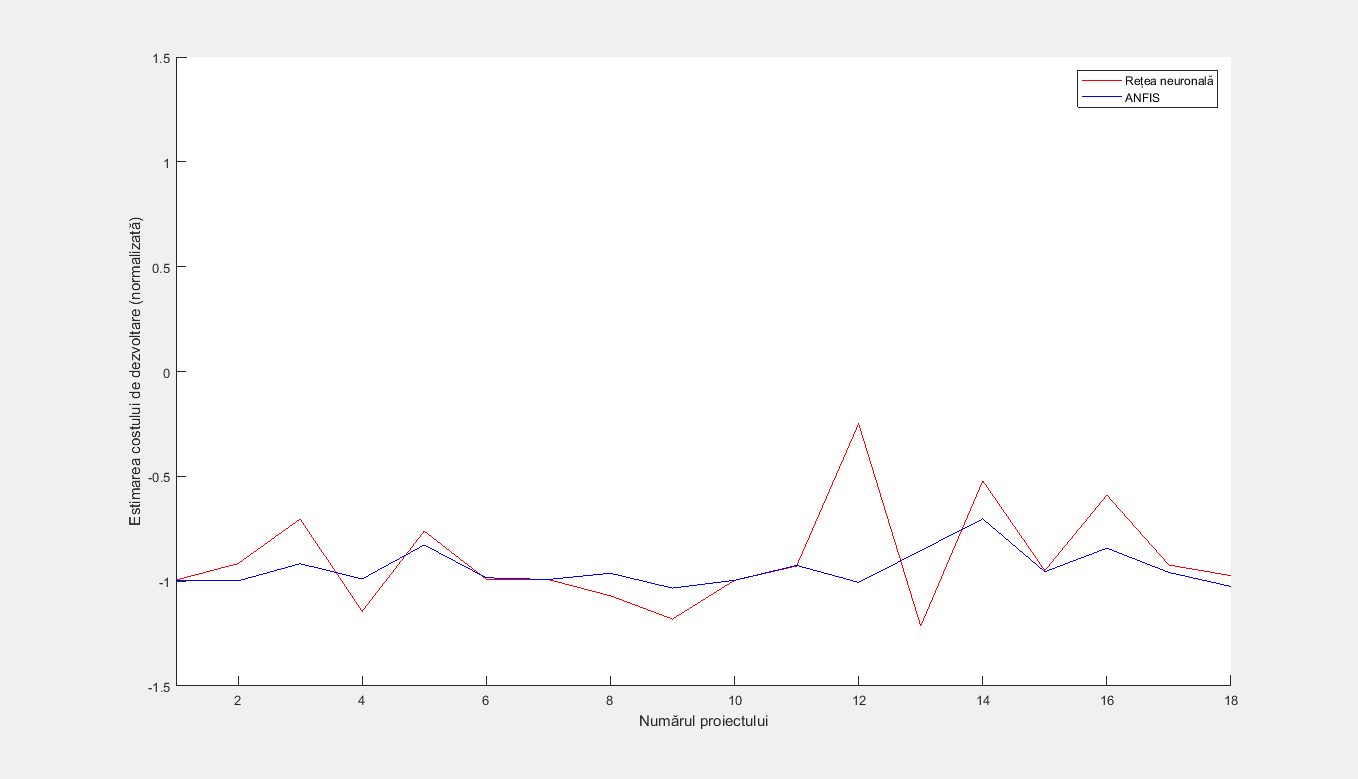
\includegraphics[width=\textwidth]{comparison}
\caption{ANFIS vs re'teaua neuronal;a peste datele de test}
\end{figure}
\par
Din figura 11.1 putem observa faptul c;a 'in afar;a de proiectele 12 'si 13, unde re'teaua neuronal;a ofer;a o estimare complet diferit;a fa't;a de ANFIS, 'in general, re'teaua neuronal;a urmeaz;a trendul ANFIS dar mult mai exagerat, 'intocmai datorit;a unor ponderi prea mari.